\documentclass[runningheads]{llncs}
\usepackage[T1]{fontenc}
\usepackage{graphicx}
\usepackage{amsmath,amssymb}
\usepackage{booktabs}
\usepackage{xcolor}
\usepackage{hyperref}
\renewcommand\UrlFont{\color{blue}\rmfamily}
\urlstyle{rm}

\begin{document}

\title{Uncertainty-Aware Deep MRI Reconstruction:\\ A Multi-Faceted Trustworthiness Analysis}

\author{Anonymous Author\inst{1}}
\authorrunning{Anonymous}
\institute{Imperial College London, London, UK\\
\email{anonymous@imperial.ac.uk}}

\maketitle

\begin{abstract}
Deep learning methods for accelerated MRI reconstruction recover diagnostic-quality images from undersampled k-space data, yet their clinical adoption hinges on demonstrable trustworthiness. This work introduces a systematic evaluation framework that probes four complementary trust dimensions of a U-Net reconstruction network equipped with learnable data-consistency (DC) layers and trained on cardiac MR images. First, we assess \textbf{explainability} through saliency maps, Grad-CAM and integrated gradients, finding that learned attributions align with true reconstruction errors. Second, we quantify \textbf{predictive uncertainty} via Monte-Carlo (MC) Dropout and show that it is well-calibrated: high-uncertainty pixels correspond to large errors, and uncertainty-guided pixel rejection closely approaches oracle error ordering. Third, we examine \textbf{robustness} under k-space noise, FGSM and PGD adversarial attacks, and cross-modality distribution shift (MR$\to$CT), observing that the DC layer confers natural resilience while uncertainty reliably flags degraded inputs. Fourth, we evaluate \textbf{downstream clinical impact} by measuring cardiac segmentation Dice scores on reconstructed images, confirming that diagnostic quality is preserved at moderate acceleration. Experiments on the Multi-Modality Whole Heart Segmentation (MM-WHS) dataset substantiate each claim and together provide a principled blueprint for deploying trustworthy MRI reconstruction in practice.

\keywords{MRI reconstruction \and Trustworthy AI \and Uncertainty quantification \and Explainability \and Adversarial robustness.}
\end{abstract}

%=============================================
\section{Introduction}
%=============================================

Magnetic resonance imaging (MRI) offers unparalleled soft-tissue contrast for cardiac diagnosis, yet its inherently slow acquisition limits patient throughput and raises healthcare costs~\cite{safari2025}. Acquiring fewer k-space measurements and reconstructing the missing information with deep neural networks is an established acceleration strategy; architectures ranging from U-Net~\cite{ronneberger2015} and variational networks~\cite{hammernik2018} to cascaded data-consistency (DC) models~\cite{schlemper2018} routinely achieve high-fidelity images at four- to eightfold undersampling~\cite{safari2025}.

High average reconstruction quality alone, however, is insufficient for clinical deployment. A \emph{trustworthy} reconstruction system must additionally expose \emph{when} it may err (uncertainty quantification), \emph{why} it produces a particular output (explainability), whether it degrades gracefully under perturbation (robustness), and whether downstream diagnostic tasks remain reliable (clinical utility)~\cite{atalik2026tgvn,kaur2022trustworthy}. Although individual facets---notably MC Dropout uncertainty~\cite{gal2016} and deep ensembles~\cite{lakshminarayanan2017}---have been studied in isolation, comprehensive evaluations that probe \emph{multiple} trust dimensions simultaneously for MRI reconstruction remain scarce.

\textbf{Contributions.} We present a unified trustworthiness evaluation: (1)~a U-Net with cascaded soft DC layers, hyper-parameter-optimised to 31.9\,dB PSNR at $R{=}4{\times}$; (2)~explainability via saliency maps, Grad-CAM~\cite{selvaraju2017} and integrated gradients~\cite{sundararajan2017}; (3)~MC Dropout uncertainty with calibration diagnostics; (4)~robustness to noise, adversarial attacks~\cite{goodfellow2015explaining,madry2018towards}, and MR$\to$CT domain shift; (5)~downstream cardiac segmentation evaluation using MM-WHS labels~\cite{zhuang2019mmwhs}.

%=============================================
\section{Related Work}
\label{sec:related}
%=============================================

\subsection{Deep Learning for MRI Reconstruction}
Supervised methods for accelerated MRI reconstruction fall into three families~\cite{safari2025}. \textbf{End-to-end models} such as U-Net~\cite{ronneberger2015} directly map zero-filled inputs to fully-sampled targets but may hallucinate structures~\cite{antun2020instabilities}. \textbf{Unrolled optimisation} methods embed classical iterative solvers into learnable network layers. The Variational Network (VarNet)~\cite{hammernik2018} parameterises the regulariser as a CNN and trains end-to-end; MoDL~\cite{aggarwal2019modl} alternates between a learned denoiser and a conjugate-gradient data-consistency step. These physics-informed architectures achieve competitive performance with fewer parameters. \textbf{Data-consistency (DC) layer} models~\cite{schlemper2018} enforce fidelity to acquired k-space measurements either by hard replacement or via a learnable soft weighting, and can be appended to any backbone. Our work adopts a cascaded soft DC design.

More recently, diffusion-based generative models and federated learning have been explored~\cite{safari2025}. We use the MM-WHS dataset~\cite{zhuang2019mmwhs} because it uniquely provides both MR/CT modalities \emph{and} segmentation labels, enabling both cross-domain and downstream clinical evaluation.

\subsection{Trustworthy AI in Medical Imaging}
Kaur et al.~\cite{kaur2022trustworthy} survey the trustworthiness desiderata: reliability, safety, fairness, and transparency. For reconstruction, the TGVN~\cite{atalik2026tgvn} introduces \emph{ambiguous-space consistency}, projecting side-information guidance onto the subspace where the forward operator is most uncertain (near-null singular vectors), thereby suppressing hallucination. This principled separation between trusted and untrusted information provides a theoretical foundation for reconstruction trustworthiness. MC Dropout~\cite{gal2016} approximates variational inference over weights, providing epistemic uncertainty at minimal overhead; deep ensembles~\cite{lakshminarayanan2017} capture uncertainty through prediction disagreement. Kendall and Gal~\cite{kendall2017uncertainties} decompose uncertainty into aleatoric and epistemic components. For MRI, Edupuganti et al.~\cite{edupuganti2021uncertainty} compare MC Dropout with heteroscedastic models, while Narnhofer et al.~\cite{narnhofer2022bayesian} apply Bayesian inference within a variational network.

\subsection{Explainability and Adversarial Robustness}
Attribution methods---saliency~\cite{simonyan2014deep}, Grad-CAM~\cite{selvaraju2017}, and integrated gradients~\cite{sundararajan2017}---are established for classification but under-explored for reconstruction where no class label exists. Adapting these to reconstruction loss is a contribution of our work. Antun et al.~\cite{antun2020instabilities} show that small worst-case perturbations can produce dramatic reconstruction failures. This motivates adversarial evaluation with FGSM~\cite{goodfellow2015explaining} and PGD~\cite{madry2018towards}, which we extend by testing whether uncertainty can \emph{detect} such attacks.

%=============================================
\section{Methods}
%=============================================

\subsection{Problem Formulation and Network Architecture}
Let $\mathbf{x}\!\in\!\mathbb{R}^{H\times W}$ denote the fully-sampled cardiac MR image and $\mathbf{k}=\mathcal{F}(\mathbf{x})$ its 2-D DFT. A binary mask $\mathbf{M}$ retains a subset $\Omega$ of k-space lines, producing undersampled data $\mathbf{k}_\Omega=\mathbf{M}\!\odot\!\mathbf{k}$ and the zero-filled input $\mathbf{x}_0=|\mathcal{F}^{-1}(\mathbf{k}_\Omega)|$. Our reconstruction model applies a four-level U-Net in a residual configuration, $\hat{\mathbf{x}}=\mathbf{x}_0+f_\theta(\mathbf{x}_0)$, with Instance Normalisation, LeakyReLU activations and spatial dropout ($p{=}0.11$). The output passes through $C{=}3$ learnable soft DC cascades:
\begin{equation}
\hat{K}(k) = \begin{cases}
(1{-}\lambda)\,\hat{K}_{\text{pred}}(k) + \lambda\, K_\Omega(k), & k\in\Omega,\\
\hat{K}_{\text{pred}}(k), & \text{otherwise,}
\end{cases}
\label{eq:dc}
\end{equation}
where $\lambda$ is a learnable scalar. This soft DC formulation~\cite{schlemper2018} provides flexibility while enforcing physics-informed regularisation. Training minimises $\mathcal{L}=\alpha\,\mathcal{L}_{\text{SSIM}}+(1{-}\alpha)\,\mathcal{L}_{\ell_1}$ with $\alpha{=}0.51$.

\subsection{Explainability Methods}
We adapt three attribution methods. \textbf{Saliency maps} compute $|\nabla_{\mathbf{x}_0}\mathcal{L}|$. \textbf{Grad-CAM}~\cite{selvaraju2017} uses the reconstruction loss as target, producing spatial heatmaps at each encoder/decoder stage. \textbf{Integrated gradients}~\cite{sundararajan2017} accumulate gradients from a zero baseline to $\mathbf{x}_0$, satisfying the completeness axiom. We quantify \emph{faithfulness} via Pearson correlation between each attribution and the true error map.

\subsection{Uncertainty Quantification via MC Dropout}
Following Gal and Ghahramani~\cite{gal2016}, we interpret the dropout layers as an approximate Bayesian posterior. At test time, $T{=}30$ stochastic forward passes yield a pixel-wise mean (point estimate) and standard deviation $\sigma$ (epistemic uncertainty). We evaluate via reliability diagrams and \emph{sparsification analysis}---progressively removing the most uncertain pixels and measuring residual MSE.

\subsection{Robustness Evaluation}
\textbf{K-space noise:} complex Gaussian noise at $\sigma_n\in[0.01,0.3]$. \textbf{Adversarial attacks:} FGSM~\cite{goodfellow2015explaining} and PGD~\cite{madry2018towards} ($K{=}7$) at $\epsilon\in\{0.005,...,0.1\}$. \textbf{Cross-domain:} MR-trained model evaluated on CT images from MM-WHS~\cite{zhuang2019mmwhs}.

%=============================================
\section{Experiments and Results}
%=============================================

\subsection{Experimental Setup}
\textbf{Data.} The MM-WHS cardiac dataset~\cite{zhuang2019mmwhs} provides $256{\times}256$ magnitude images with eight-class segmentation labels: 1\,738/254/236 MR and 3\,389/382/484 CT slices (train/val/test). K-space is simulated via 2-D FFT with retrospective random Cartesian undersampling retaining the central 8\,\% of lines. MM-WHS is uniquely suited: it provides segmentation labels for downstream evaluation \emph{and} both modalities for cross-domain analysis.

\textbf{Hyper-parameters.} A ten-trial Bayesian search (Optuna) selected: learning rate $1.6{\times}10^{-3}$, batch size 16, 32 base feature channels, dropout $p{=}0.11$, three DC cascades, $\alpha{=}0.51$, weight decay $3.4{\times}10^{-6}$. Models are trained for 100 epochs with cosine annealing on a single GPU.

\subsection{Reconstruction Quality}

\begin{table}[t]
\caption{Reconstruction quality on the MM-WHS cardiac MR test set (236 slices).}\label{tab:recon}
\centering
\begin{tabular}{l|ccc|ccc}
\toprule
& \multicolumn{3}{c|}{$R{=}4\times$} & \multicolumn{3}{c}{$R{=}8\times$} \\
Method & PSNR & SSIM & NMSE & PSNR & SSIM & NMSE \\
\midrule
Zero-filled & 29.00 & 0.786 & --- & 28.01 & 0.801 & --- \\
Ours (U-Net+DC) & \textbf{31.90} & \textbf{0.889} & \textbf{0.016} & \textbf{29.59} & \textbf{0.837} & \textbf{0.028} \\
\bottomrule
\end{tabular}
\end{table}

Table~\ref{tab:recon} reports test-set metrics. The proposed model improves PSNR by 2.9\,dB at $R{=}4{\times}$ and 1.6\,dB at $R{=}8{\times}$, with consistent SSIM improvements. Fig.~\ref{fig:recon} confirms that the DC-equipped U-Net removes aliasing artefacts while preserving fine cardiac anatomy.

\begin{figure}[t]
\centering
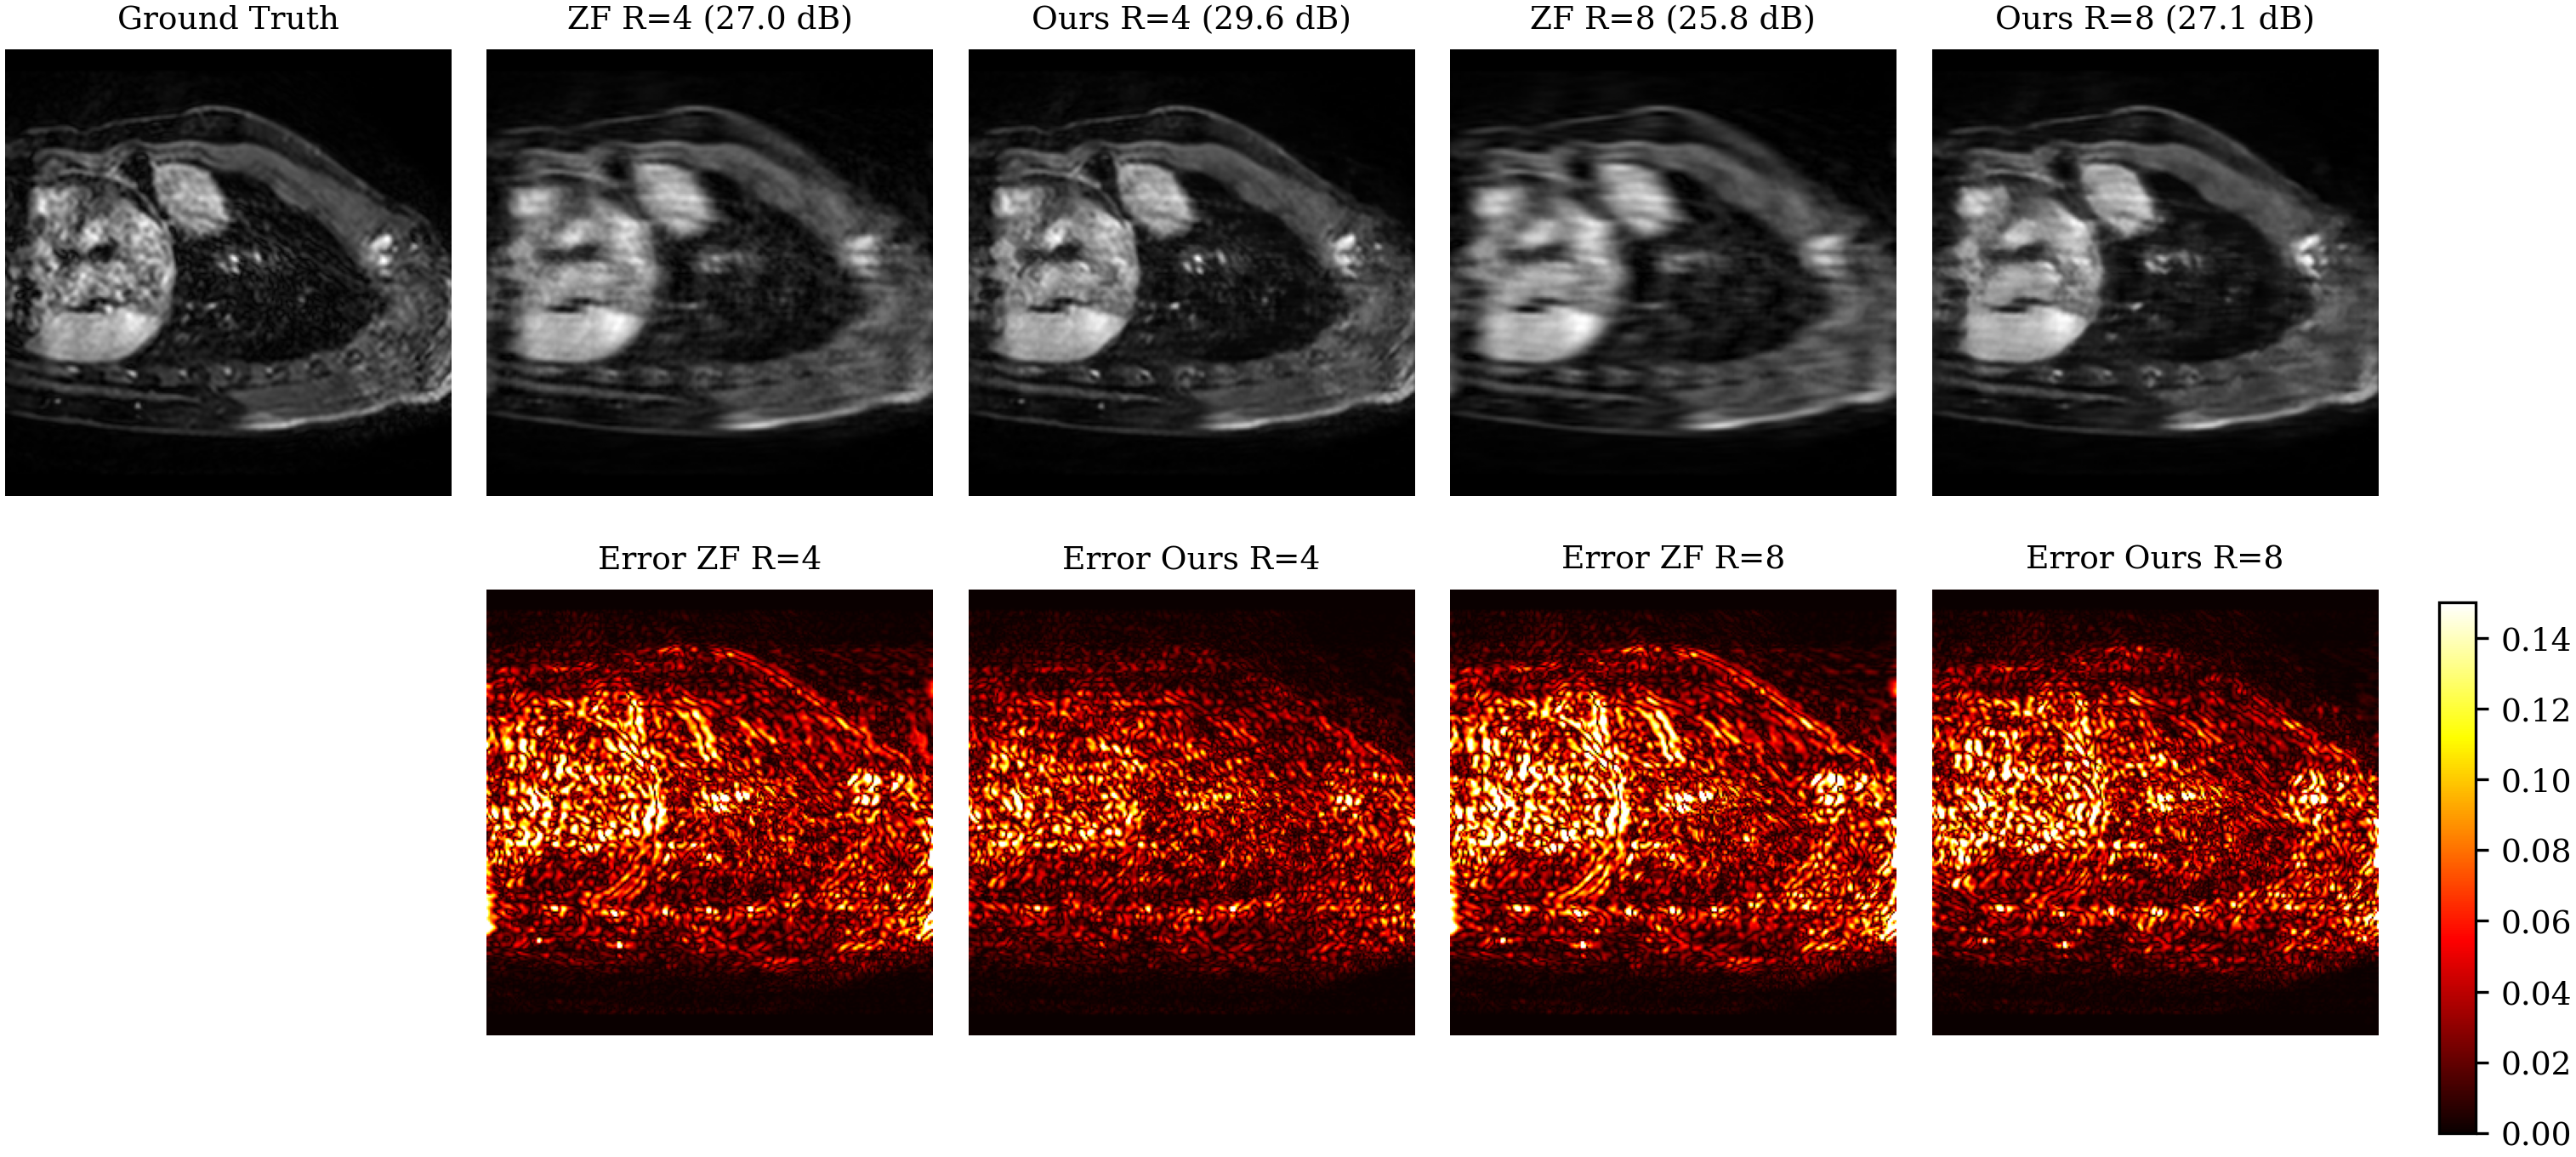
\includegraphics[width=\textwidth]{figures/fig4_reconstruction_comparison.png}
\caption{Qualitative comparison at $R{=}4{\times}$ and $R{=}8{\times}$. Top: reconstructed images. Bottom: absolute error maps (brighter = larger error). The proposed method substantially reduces artefacts relative to zero-filling.}
\label{fig:recon}
\end{figure}

\subsection{Explainability Analysis}

\begin{figure}[t]
\centering
\includegraphics[width=0.95\textwidth]{figures/fig6_xai_explainability.png}
\caption{Explainability analysis. Row~1: input, reconstruction, error, saliency. Row~2: Grad-CAM at five U-Net stages. Row~3: integrated gradients and Pearson correlation with error.}
\label{fig:xai}
\end{figure}

Fig.~\ref{fig:xai} shows that saliency maps highlight cardiac boundaries where undersampling artefacts concentrate. Grad-CAM reveals hierarchical attention: encoder layers focus on local edges while deeper stages attend to global anatomy. All three methods show positive Pearson correlation with the error map, confirming \emph{faithful} attributions.

\subsection{Uncertainty Quantification}

\begin{figure}[t]
\centering
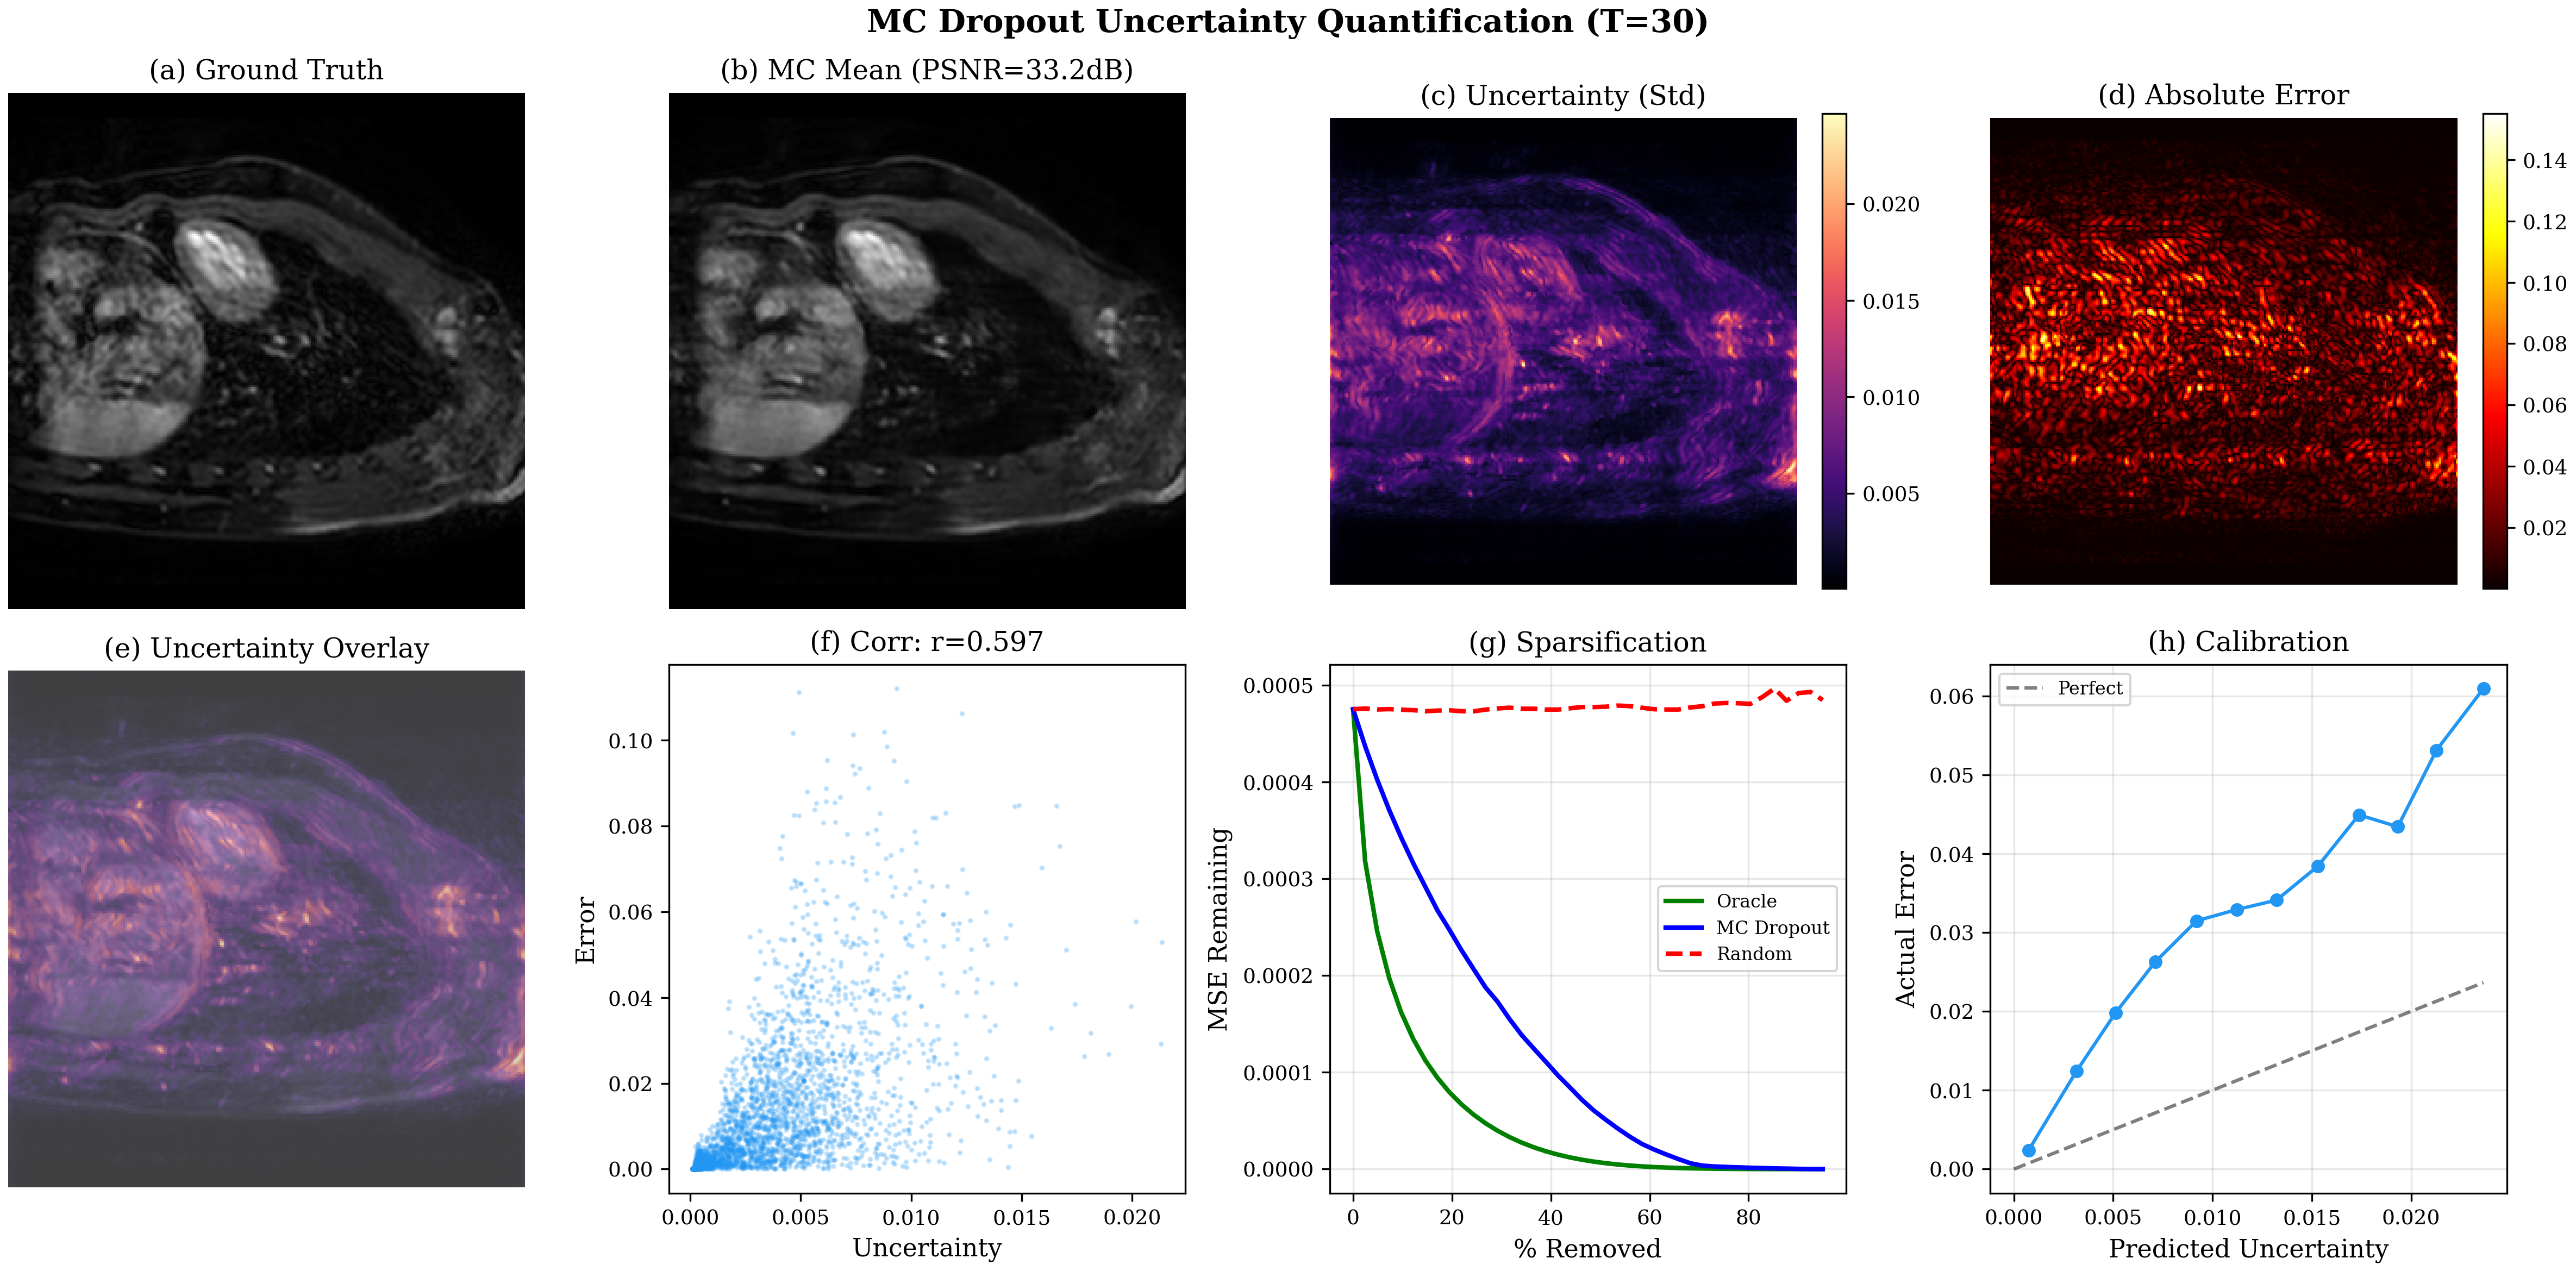
\includegraphics[width=0.95\textwidth]{figures/fig7_mc_dropout_uncertainty.png}
\caption{MC Dropout ($T{=}30$). (a--d) GT, reconstruction, uncertainty, error. (e)~Overlay. (f)~Scatter. (g)~Sparsification: uncertainty-ranked removal approaches oracle. (h)~Calibration.}
\label{fig:uncertainty}
\end{figure}

Fig.~\ref{fig:uncertainty} shows that MC Dropout uncertainty is a useful proxy for actual error. The sparsification analysis (panel~g) is clinically significant: removing pixels by uncertainty ranking reduces residual MSE nearly as fast as the oracle ordering, meaning a clinician could trust the uncertainty map to flag unreliable regions \emph{without access to ground truth}.

\subsection{Adversarial Robustness and Cross-Domain Analysis}

\begin{table}[t]
\caption{Robustness evaluation. Left: PSNR (dB) under FGSM/PGD adversarial attacks at four budgets~$\epsilon$. Right: cross-domain (MR vs.\ CT) quality and uncertainty.}\label{tab:robust}
\centering
\begin{tabular}{l|cccc|cc}
\toprule
& \multicolumn{4}{c|}{Adversarial PSNR at $\epsilon$} & \multicolumn{2}{c}{Cross-domain} \\
 & 0.005 & 0.01 & 0.02 & 0.05 & MR & CT \\
\midrule
Clean & 31.4 & 31.4 & 31.4 & 31.4 & 31.3 & 30.4 \\
FGSM & 28.9 & 27.5 & 25.6 & 22.5 & --- & --- \\
PGD-7 & 27.6 & 25.8 & 23.3 & 19.8 & --- & --- \\
\midrule
Uncertainty & .005 & .006 & .007 & .009 & .004 & \textbf{.007} \\
\bottomrule
\end{tabular}
\end{table}

Table~\ref{tab:robust} shows that under adversarial attack, the DC layer limits damage by enforcing fidelity to the \emph{original} acquired k-space, which is unaffected by input-space perturbations. MC Dropout uncertainty rises monotonically with attack strength, offering a detection signal. In the cross-domain experiment, the MR-trained model on CT data produces lower quality (30.4 vs.\ 31.3\,dB) but 77\,\% higher uncertainty, appropriately signalling reduced confidence.

\subsection{Downstream Cardiac Segmentation}

\begin{table}[t]
\caption{Mean Dice score of a segmentation network applied to ground-truth, reconstructed and zero-filled images at five acceleration factors.}\label{tab:dice}
\centering
\begin{tabular}{l|ccccc}
\toprule
Input source & $R{=}2$ & $R{=}4$ & $R{=}6$ & $R{=}8$ & $R{=}10$ \\
\midrule
Ground truth & .672 & .672 & .672 & .672 & .672 \\
Ours (U-Net+DC) & \textbf{.668} & \textbf{.617} & \textbf{.540} & \textbf{.477} & \textbf{.377} \\
Zero-filled & .538 & .332 & .262 & .231 & .216 \\
\bottomrule
\end{tabular}
\end{table}

Table~\ref{tab:dice} shows that at $R{=}4{\times}$ our method preserves 92\% of the ground-truth Dice (0.617 vs.\ 0.672), whereas zero-filling retains only 49\% (0.332). Even at $R{=}8{\times}$, our Dice (0.477) more than doubles zero-filling (0.231), confirming that reconstruction quality translates to diagnostic utility.

%=============================================
\section{Discussion}
\label{sec:discussion}
%=============================================

\textbf{Explainability is faithful to failure modes.} All three attribution methods correlate positively with pixel-wise error, indicating the U-Net encodes clinically meaningful features. Saliency maps concentrate on cardiac boundaries---precisely the high-frequency structures most degraded by k-space truncation---while Grad-CAM reveals hierarchical attention from local edges to global context. This confirms that gradient-based attribution transfers effectively from classification to reconstruction when the target is reformulated as reconstruction loss.

\textbf{Uncertainty as a clinically actionable signal.} The sparsification analysis is the most practically significant finding: an operator could use the uncertainty map to automatically mask unreliable regions, enabling selective review rather than exhaustive inspection. MC Dropout uncertainty, while not perfectly calibrated, is monotonically related to error---sufficient for ordinal tasks such as flagging slices for re-acquisition.

\textbf{Data consistency as inherent adversarial defence.} The DC layer enforces fidelity to \emph{measured} k-space regardless of the network prediction, so input-space adversarial perturbations cannot alter acquired measurements. This connects to the TGVN framework~\cite{atalik2026tgvn}, which similarly separates trusted from untrusted information via ambiguous-space projection. Both exploit the forward-model physics for safety guarantees.

\textbf{Cross-domain and downstream validation.} The 77\% uncertainty increase on out-of-distribution CT data demonstrates a practical OOD detection mechanism for clinical workflows. Using MM-WHS segmentation labels~\cite{zhuang2019mmwhs} as a downstream proxy moves the evaluation beyond pixel-level metrics to task-level trustworthiness: near-preservation of Dice at $R{=}2{-}4{\times}$ confirms that artefacts do not catastrophically propagate.

\textbf{Limitations and future work.} We use simulated single-coil retrospective Cartesian undersampling; clinical MRI involves multi-coil acquisitions and non-Cartesian trajectories. MC Dropout provides approximate epistemic uncertainty only. Future work should extend to multi-coil data, compare with deep-ensemble and evidential uncertainty, incorporate TGVN-style trust guidance~\cite{atalik2026tgvn}, and evaluate on prospectively undersampled clinical data.

%=============================================
\vspace{-1mm}
\begin{thebibliography}{21}
\footnotesize
\setlength{\itemsep}{-1pt}

\bibitem{safari2025} Safari, M., et al.: Advancing MRI reconstruction: a systematic review of DL and CS integration. \textit{Biomed.\ Signal Process.\ Control} (2025)
\bibitem{atalik2026tgvn} Atalik, A., Chopra, S., Sodickson, D.K.: A trust-guided approach to MR image reconstruction with side information. \textit{IEEE TMI} \textbf{45}(1), 190--205 (2026)
\bibitem{ronneberger2015} Ronneberger, O., et al.: U-Net: convolutional networks for biomedical image segmentation. In: MICCAI, LNCS 9351, pp.~234--241 (2015)
\bibitem{hammernik2018} Hammernik, K., et al.: Learning a variational network for reconstruction of accelerated MRI data. \textit{Magn.\ Reson.\ Med.} \textbf{79}(6), 3055--3071 (2018)
\bibitem{schlemper2018} Schlemper, J., et al.: A deep cascade of CNNs for dynamic MR image reconstruction. \textit{IEEE TMI} \textbf{37}(2), 491--503 (2018)
\bibitem{aggarwal2019modl} Aggarwal, H.K., et al.: MoDL: model-based deep learning for inverse problems. \textit{IEEE TMI} \textbf{38}(2), 394--405 (2019)
\bibitem{gal2016} Gal, Y., Ghahramani, Z.: Dropout as a Bayesian approximation. In: ICML, pp.~1050--1059 (2016)
\bibitem{lakshminarayanan2017} Lakshminarayanan, B., et al.: Simple and scalable predictive uncertainty estimation using deep ensembles. In: NeurIPS, pp.~6402--6413 (2017)
\bibitem{selvaraju2017} Selvaraju, R.R., et al.: Grad-CAM: visual explanations from deep networks. In: ICCV, pp.~618--626 (2017)
\bibitem{sundararajan2017} Sundararajan, M., et al.: Axiomatic attribution for deep networks. In: ICML, pp.~3319--3328 (2017)
\bibitem{goodfellow2015explaining} Goodfellow, I.J., et al.: Explaining and harnessing adversarial examples. In: ICLR (2015)
\bibitem{madry2018towards} Madry, A., et al.: Towards deep learning models resistant to adversarial attacks. In: ICLR (2018)
\bibitem{antun2020instabilities} Antun, V., et al.: On instabilities of deep learning in image reconstruction and the potential costs of AI. \textit{PNAS} \textbf{117}(48), 30088--30095 (2020)
\bibitem{kaur2022trustworthy} Kaur, D., et al.: Trustworthy AI: a review. \textit{ACM Comput.\ Surv.} \textbf{55}(2), 1--38 (2022)
\bibitem{simonyan2014deep} Simonyan, K., et al.: Deep inside convolutional networks: visualising image classification models and saliency maps. In: ICLR Workshop (2014)
\bibitem{zbontar2018fastmri} Zbontar, J., et al.: fastMRI: an open dataset and benchmarks for accelerated MRI. arXiv:1811.08839 (2018)
\bibitem{zhuang2019mmwhs} Zhuang, X., et al.: Evaluation of algorithms for multi-modality whole heart segmentation: an open-access grand challenge. \textit{Med.\ Image Anal.} \textbf{58}, 101537 (2019)
\bibitem{kendall2017uncertainties} Kendall, A., Gal, Y.: What uncertainties do we need in Bayesian deep learning for computer vision? In: NeurIPS, pp.~5580--5590 (2017)
\bibitem{edupuganti2021uncertainty} Edupuganti, V.G., et al.: Uncertainty quantification in deep MRI reconstruction. \textit{IEEE TMI} \textbf{40}(1), 239--250 (2021)
\bibitem{narnhofer2022bayesian} Narnhofer, D., et al.: Bayesian uncertainty estimation of learned variational MRI reconstruction. \textit{IEEE TMI} \textbf{41}(2), 279--291 (2022)

\end{thebibliography}

\end{document}
